\documentclass[]{article}
\usepackage{amsmath}
\usepackage{amssymb}
\usepackage{graphicx}

\title{Physics 229}
% \author[1]{Andrew MacRae}
% \affil[1]{D of P and A, U of V}
\begin{document}
\section{Amplifiers}
\subsection{Active vs. Passive Circuits}
We now move into the regime of so-called \textit{active electronics}. Everything studied so far -- resistors and capacitors, to voltage dividers and filters, to diode rectifiers has fallen under the realm of passive electronics. Active electronic devices, in addition to standard inputs and outputs, require additional power supplies in order to function. There are great benefits to this, as we shall see: active components can output more power than at their input, and can eliminate annoying effects such as voltage loading due to input and output impedance. The first active device we'll study is the amplifier.
\subsection{The Ideal Voltage Amplifier}
The idea of the basic amplifier is simple: take the input $x_\text{in}$ and produce an output which is some number $G$ times the output.
\begin{equation}
\label{eq:simple_amp}
x_\text{out} = Gx_\text{in}
\end{equation}

\noindent ... where $G$ is known as the gain.

There is the question of what input $x_\text{in}$ is being amplified. In our course, normally $x_\text{in}$ will be a voltage and so we will have a voltage amplifier. In this case the gain is often expressed in decibals as:

\begin{equation}
\label{eq:voltage_amp_dB}
G_\text{dB} = 20\log\frac{v_\text{out}}{v_\text{in}} 
\end{equation}

We will occasionally deal with power amplifiers whose input and output is a power. For these amplifiers, the gain is also in dB but with a 10 instead of a 20 multiplier\footnote{Recall that for a fixed load resistance, $P = v^2/R \propto v^2$. Thus $10\log\left[P_\text{out}/P\text{in}\right] = 10\log\left[\left(v_\text{out}/v\text{in}\right)^2\right] = 20\log\left[v_\text{out}/v_\text{in}\right]$, thus yielding consistant definitions of gain}:

\begin{equation}
\label{eq:power_amp_dB}
G_\text{dB} = 10\log\frac{P_\text{out}}{P_\text{in}} 
\end{equation}

\noindent For now though, we will restrict outselves to voltage amplifiers. Diagrammed in figure \ref{fig:simple_amp}. The output is descibed by equation \ref{eq:simple_amp}.

\begin{figure}[h]
\caption{The simplest of amplifiers: the output is the input multiplied by a constant gain $G$.}
\label{fig:simple_amp}
\begin{center}
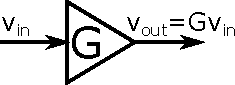
\includegraphics{Images/SimpleAmplifier.pdf}
\end{center}
\end{figure}

\subsection{Reality Check: Amplifiers in Real Life}
There are several limitations to the ideal amplifier that come into effect in practice. For example the amplifier will have to draw at least a small current from the source in order to operate. As we've learned, this is equivalent to a finite \textit{input impedance} $R_\text{in}$. The amplifier will also have a limit to how much current it can output due to its internal resistances. This leads to a finite \textit{output impedance} $R_{out}$. There are also limits to how fast the amplifier can respond to a changing input signal. This leads to a finite \textit{gain bandwidth}, or in general, a frequency dependant gain $G(\omega)$. We will examine each of these effects presently.

\subsection{Effects of Finite Input Impedance}
\label{sec:AMP_effect_input}
We can model the non-ideal amplifier as an ideal amplifier inside a black box, precisely as we did with ideal vs real voltage sources. Inside the black-box, the input impedance is models as an internal resistance $R_\text{in}$ to ground placed before the ideal amplifier. This forms a voltage divider with the input impedance from the rest of the circuit so that there is some voltage drop. The ideal amplifier thus sees a different voltage than $v_\text{in}$, which we denote $v^\prime_\text{in}$. The output of the real amplifier is thus less than we would expect: $v_\text{out} = Gv^\prime_\text{in} < Gv_\text{in}$
\begin{figure}[h]
\caption{We model the finite input impedance of the amplifier as a internal resistor $R_\text{in}$ to ground before an ideal amplifier all in a black box.}
\label{fig:real_amp_int}
\begin{center}
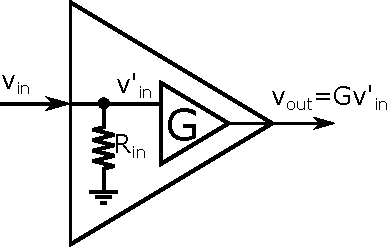
\includegraphics{Images/RealAmplifier_int.pdf}
\end{center}
\end{figure}

The true output, given the input impedance can be calculated given the output impedance of whatever follows. For example, with a $100$~$\Omega$ input impedance amplifier with $G = 10$, 

\subsection{Effects of Finite Output Impedance}
The operation of our ideal amplifier can be seen as a two part process: first it senses the voltage at its input (with the effect of finite input impedance causing some loading error), and second, it acts as a new voltage source, producing a voltage $v_\text{out} Gc_\text{in}$. As with any \textit{real} source, it will be equivalent to an ideal source, in series with an output impedance $R_\text{out}$. This finite output impedance leads to a maximum short-circuit current of $v_\text{out}/R_\text{out}$ and will lead to all of the loading issues discussed in chapter XXX. Figure \ref{fig:real_amp_int_out} shows our improved model of how a real amplifier behaves.
\begin{figure}[h]
\caption{A better model of a real amplifier has an input resistance to ground in parallel with the inpput and an output resistance in series with its output.}
\label{fig:real_amp_int_out}
\begin{center}
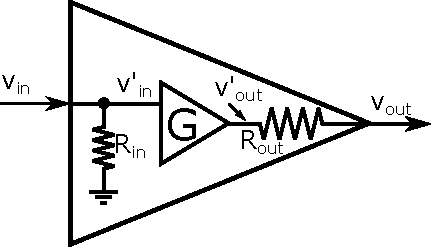
\includegraphics{Images/RealAmplifier_int_out.pdf}
\end{center}
\end{figure}

\noindent\textbf{Design Example:} Consider a real amplifier with $R_\text{in} = 10$~k$\Omega$, $R_\text{F} = 100~\Omega$, and G = 25. We use it to amplify a 10~mV signal from a photodetector having $R_\text{out,PD} = 1250~\Omega$ and send it to a (lousy) voltmeter with $R_\text{in,LVM}$ = 500~$\Omega$ (see figure \ref{fig:prob_amp}). What is the voltage measured (a) assuming an ideal $G = 25$ amplifier, and (b) with our real amplifier?\\\\\noindent Answer: For part (a) the answer is simply $v_\text{meas} = 25\times10~$mV = 250~mV. For our real amplifier, we must consider the input and output stage. The input now forms a voltage divider with $R_\text{in}$ (figure \ref{fig:prob_amp}b so that the inner ideal amplifier sees:
$$
v_\text{in}^\prime=\frac{R_\text{in}}{R_\text{out,PD} + R_\text{in}} = \frac{10~\text{k}\Omega}{11.25~\text{k}\Omega}\times10~\text{mV} \approx 8.9~\text{mV}
$$
In our model, this is then amplified by the ideal internal amplifier producing
$$
v_\text{out}^\prime = 8.9~\text{mV}\times 25 \approx 222~\text{mV}
$$
Finally, this is then sent to our lousy voltmeter, through its internal output resistance, forming another voltage divider (figure \ref{fig:prob_amp}c) to yeild the final voltage:
$$
v_\text{out} = \frac{R_\text{in,LVM}}{R_\text{out} + R_\text{in,LVM}}v_\text{out}^\prime = \frac{500~\Omega}{600~\Omega}\times 222~\text{mV}\approx 185~\text{mV}
$$

\begin{figure}[ht]
\caption{Example Problem.}
\label{fig:prob_amp}
\begin{center}
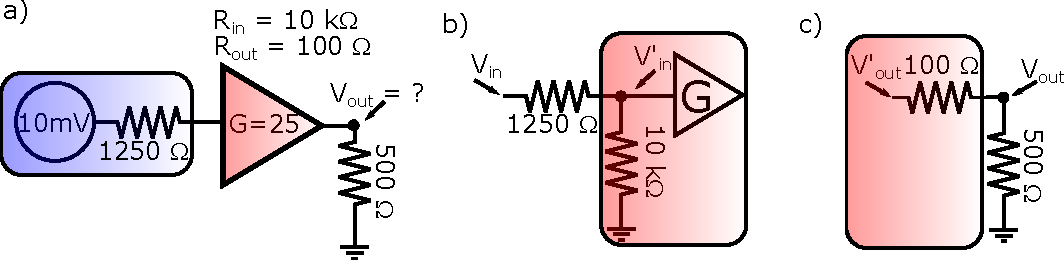
\includegraphics[width=\textwidth]{Images/amp_example.pdf}
\end{center}
\end{figure}

We thus see that the effect of finite input and output impedance is to lessen the effective gain of the real amplifier. Even if we used an ideal voltmeter with infinite input impedance, we'd still see 222~mV $<$ 250~mV. Equivalently, we could try to build an amplifier with $R_\text{out} \rightarrow 0~\Omega$ and again we'd see 222~mV, regardless of the impedance of the voltmeter. To get the full 250~mV however, we'd need to also have $R_\text{in} \rightarrow \infty$, so that $v_\text{in}^\prime = v_\text{in} = 25$~mV. 

From this we can infer the ideal characteristrics of a real amplifier: we want the input impedance as high as possible while having output impedance as low as possible. This can be accomplished using solid state transistors, discussed later in the course. 

\subsection{Effects of Noise: Noise Factor and SNR}
The ideal amplifier will amplify the voltage present at it's input, regardless of whether we consider that voltage to be useful signal or to be noise. This can lead to fundamental issues in isolating very weak signals since eventually, we will just be scaling up Johnson, Shot, or technical noise. 

For example, if you have a 10~nV signal atop 25~nV of Johnson noise, you can send your signal to a 120~dB amplifier to get 100~mV of signal, but it will still be lost in the Johnson noise, which is now at 250~mV.  We amplified the signal level, but have not improved the signal level as compared to the signal. This ratio of signal vs noise has, in a spark of linguistic creativity, been dubbed the ``signal to noise ratio'' or SNR. since the voltage of the noise is usually stochastic \footnote{ A high-brow term, effectively meaning ``random''}, usually the signal to noise ratio is usually specified in terms of power, rather than voltage\footnote{ ...wait, what $R$ should we use here? Well power is energy per unit time and that energy has to be delivered to something. That something is the load resistance, so that a given voltage noise will deliver more power to a 1$00~\Omega$ than a $100~\text{k}\Omega$ resistor} (ie. $v_{RMS}^2/R)$

\begin{equation}
\label{eq:def_snr}
\text{SNR} \equiv \frac{P_\text{sig}}{P_\text{noise}} = 10\log_{10}\left[\frac{P_\text{sig}}{P_\text{noise}}\right] \text{dB}
\end{equation}

So an amplifier on its own will not help you discern signals dominated by noise and the SNR must be improved though separate means. If your signal exits within a given range of frequencies but your noise exists at all frequencies, a filter can be applied to the input of the amplifier to greatly improve the SNR. If the  signal and noise coexist at the same range of frequencies, you have to be more clever. For example, a common source of noise is thermal motion of electrons through a load resistance. To improve the SNR, circuits are often cooled to -40 $^\circ$C or even as low as several Kelvin, when extremely faint signals are being detected.

To make matters worse, the amplifier often adds its own noise to the system - that is the SNR of the output is typically even higher than that of the input! This is quantified by the so-called noise figure:

\begin{equation}
\label{eq:def_noise_figure}
\text{NF} \equiv \frac{\text{SNR}_\text{out}}{\text{SNR}_\text{in}} = 10\log_{10}\left[\frac{\text{SNR}_\text{out}}{\text{SNR}_\text{in}}\right]
\end{equation}

\noindent Good amplifiers will have NF $2$~dB or less.

\subsection{Effects of Finite Frequency Response}
Since every circuit element has some finite capacitance and inductance, we can replace the internal input and output resistances with an input impedance $Z_\text{in}$ and output impedance $Z_\text{out}$. The net effect of this is to produce a frequency dependant gain $G(\omega)$. This can be modelled as internal frequency filter that is applied to the input or output. This bug can be rebranded as a feature as an amplifier may actually filter out high frequency noise present in the signal, as discussed in the previous section.

\subsection{Differential Amplifiers}
\label{sec:diff_amps}
Often in physics, it is a small deviation from a fixed value that is of interest rather than the absolute value itself. For example, a beam of light may pick up a small oscillation in intensity as compared to a reference beam when passed through a sample. In this case, a \textit{differential amplifier} may be used. As diagrammed in figure XXX, a differential amplier has two inputs and a single output corresponding to the difference between the signals. This is operation can be seen as first inverting one input and then adding it to the other. The input which is inverted $V_-$ is fitting called the ``inverting input'', while the normal input is verbosely titled the ``non-inverting input'', $V_+$. The multiplication factor is known as the ``differential gain'' $G_\text{diff}$ and is defined through the relation
\begin{equation}
\label{eq:def_diff_amp}
v_\text{out} = G_\text{diff}\left(v_+-v_-\right).
\end{equation}

\textit{Example:} A differential amplifier with $G_\text{diff} = 40$~dB has, at its inputs: $v_+ = 3.7$~mV and $v_- = 4.2$~mV. What is the output voltage?\\\\
\textit{Solution:} The gain of 40~dB implies that $20\log_{10}\frac{v_\text{out}}{v_+-v_-} = 40$, so that $v_\text{out} = 100\left(v_+-v_-\right)$. Since, $\left(v_+-v_-\right) = \left(3.7-4.2\right)~\text{mV} = -0.5~\text{mV}$, we will find $v_\text{out} = -500~$mV.
\subsection{Common Mode Gain}
From equation \ref{eq:def_diff_amp}, we expect that if $v_+ = v_-$, we will have $v_\text{out} = 0$ regardless of the value of $v_+$ and $v_-$. In practice however, this is not the case. This can be due, for example, to differences in the input impedances of the individual inputs so that internally, $v_-^\prime \neq v_+^\prime$ even though $v_- = v_+$ (see the previous section \ref{sec:AMP_effect_input}). To quantify this, we define the \textit{common-mode voltage} as the average of the inverting vs. non-inverting input voltages:
\begin{equation}
\label{eq:common_mode_voltage}
v_\text{com} \equiv \frac{v_+-v_-}{2}
\end{equation}

The amount of signal that gets through defines the \textit{common-mode gain}
\begin{equation}
\label{eq:common_mode_gain}
v_\text{out} = G_\text{com}\frac{v_++v_-}{2}
\end{equation}
An ideal differntial amplifier would have $G_\text{com} = 0$ or $-\infty$~dB. The true output of the \textit{real} differential amplifier is thus:
\begin{equation}
\label{eq:real_diff_amp}
v_\text{out} = G_\text{diff}\left(v_+-v_-\right) + G_\text{com}\frac{v_++v_-}{2}.
\end{equation}

\subsection{Common Mode Rejection Ratio}
The ``goodness'' of a differential amplifier is how much it behaves like one! Mathematically we can quantify this by saying that for a good differential amp, $G_\text{com} \ll G_\text{diff}$. THis is represented by the so-called ``common-mode rejection ratio'' or CMRR. The CMRR is usually stated in decibels and is given by:
\begin{equation}
\label{eq:def_CMRR}
\text{CMRR} \equiv 20\log_{10}\left[\frac{G_\text{diff}}{G_\text{com}}\right]
\end{equation}
 
Decent differential amplifiers have CMRR$^\text{s}$ of at least 70~dB but some applications require 120~dB or higher.
%\subsection{Special Purpose Amplifiers}Power amplifiers, Audio Amplifiers, Instrumentation Amplifiers, oh my! Also Lock-In Amplifiers!

\section{Feedback and Op Amps}
By far and wide, the amplifier that you will see the most of in the labs is a very high gain, differential amplifier known as an ``operational amplifier'', or \textit{Op Amp}. Op-amps form the basis of a very wide range of applications: adding and subtracting voltages, frequency filters, low-noise single-input amplifiers, circuit protection, oscillators/fucntion generators, and analog to digital converters, (to name a few). The typical differential gain of an op-ampo is insanely high - 1,000,000 or higher. The gain is so high infact that it renders opamps useless when used as standard differential op-amps. The utility of an op-amp comes in by employing the crucial concept of negative feedback, which we will explore presently.

\subsection{Negative Feedback}
Feedback refers to a configuration in which the output of a system is connected back into its input (ie. ``fed back''). Feedback systems are everywhere in nature: in the human body the amount of insulin in the bloodstream is sensed and fed back into beta cells in the pancreas which determine the amount of insulin to be secreted. In climatology, a mechanism for ice ages is thought to be that colder weather creates more snow and thus more light is reflected back into space, creating more snow, etc. Of course, feedback systems can be engineered by us humans as well. The formal theory of feedback is a part of the field known as control theory.

A simple feedback system is shown in figure \ref{fig:simple_feedback}.

\begin{figure}[ht]
\caption{The simplest feedback system.}
\label{fig:simple_feedback}
\begin{center}
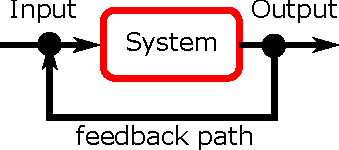
\includegraphics[]{Images/simple_feedback.pdf}
\end{center}
\end{figure}

\subsection{Op Amps in Negative Feedback: The Golden Rules}
Let's observe the operating characteristics of an ideal opamp, operating in a simple negative feedback configuration as diagrammed in figure [XXX]. We can look at both in terms of an abstract feedback system and also try to get a picture of what's going on ``under the hood''. Let's start with the former: We don't know what the output actually is, but from the definition of a differential amplifier (equation \ref{eq:def_diff_amp}), and from the fact that the output is wired to the the inverting input (hence negative feedback) we see that $v_+ = v_\text{in}$ and $v_-=\text{out}$. Thus:

\begin{equation*}
v_\text{out} \equiv G\left(v_+ - v_-\right)  = Gv_\text{in} - Gv_\text{out}
\end{equation*}

\noindent ... so that 
\begin{equation}
\label{eq:opamp_analysis_feedback}
v_\text{out} = \left(\frac{G}{G-1}\right)v_\text{in}
\end{equation}
In the limit of an ideal opamp, $G\rightarrow\infty$ so that this becomes $v_\text{out} = v_\text{in}$. Congratulations, we've just made the worlds most useless circuit. Or have we? In fact, although I chose this as a simple way to understand opamps, this circuit, known as a ``buffer op-amp'' is indeed very usefull and is found everywhere. Why? Because of the other property of the opamp - the insanely high input impedance. This means that the non-inverting opamp ``sniffs-out'' the input voltage while drawing negligable current, reproducing the voltage at the output and providing whatever current is called for. But where does this current come from if not the input? It turns out that we forgot to draw all of the opamp's terminals on our sketch - op-amps are active components and thus need power. Whatever power is needed for the output essentially comes from the power terminals and our buffer opamp thus separates whatever is on the input side of the circuit from the components on the output. We can drive large amounts of current without disturbing the sensor, voltage divider, or whatever is going into the circuit. No loading error, near zero output impedance. The buffer opamp creates a signal and converts it into a near-ideal source.

The above example illustrates the most important features of opamps in negative feedback. They are so useful in understanding how opamps behave, that they have been dubbed ``The Golden Rules of OpAmps'':
\\\\
\textbf{Golden Rule I}: The opamp draws no current at its inputs: $i_+ = i_- = 0$.
\\\\
\textbf{Golden Rule II}: In negative feedback, the opamp's output adjusts itself so that it' inputs are equal $v_+ = v_-$.

The first rule is merely a restatment that opamps have very large input impedance. The second rule is a property of negative feedback, but is less obvious than the first. To understand why it must be so, lets reanalyze the previous example in a more empirical manner. Consider again the circuit in figure [xxx]. Suppose we have just switched the circuit on and the output is some randome value (I don't know ... $-1.234$~V say) and the input is at 3~V. The input sees a voltage diference of 4.234~V and immediately starts trying to put out an enormous, positive voltage (although it can't switch instantaneously, since there's always some capacitance inductance and resistance in the circuit.) Thus a split secon later, the output difference has been reduced, say to +2V. Now the output difference is 1~V and again the output tries to become more positive (but less than before.) After a short time the output reaches +3~V and the output no longer tries to swing to a more positive value. Suppose that it overshoots 3~V (due to its small parasitic inductance) so that the voltage is now at 3.1~V. The difference voltage is now -0.1~V and the output now starts becoming negative. We see the action of negative feedback on the system -- when the output is lower than the input it quickly becomes larger and when it is higher, it quickly becomes lower. The only stable configuration is where the output equals the input. This is why \textbf{GR II} works. 

Of course, we can do much more with opamps than to create a voltage buffer. There are, quite literally, shelves in libraries filled with entire books on opamps. We'll go through the more common opamp applications in the following sections. We can use the golden rules of opamps throughout to analyze the functionality of these circuits.

\subsection{Inverting Opamps}
The next simplest opamp to analyze is the inverting opamp, seen in figure [xxx]. Here the gain is a negative number so that a positive input produced a negative output and vice versa. 

To understand the functionality of this opamp, we apply the golden rules. First, since the non-inverting output is shorted to ground \textbf{GR II} tells us that the noninverting terminal is also clamped to ground. In this situation, the node at the inverting terminal is said to be a \textit{virtual ground}. The current through the first resistor $R_1$ is thus:

\begin{equation}
\label{eq:inverting_opamp_deriv_1}
i_{R_1} = \frac{v_+}{R_1}
\end{equation}

Next, \textbf{GR I} tells us that no current runs into the $v_+$ terminal so that by Kirchhoff's rules, $i_{R_2} = i_{R_1} = v_+/R_1$. This allows us to determin the voltage drop across the second resistor $R_2$ (note now that the voltage goes from 0 to something lower):
\begin{equation}
\label{eq:inverting_opamp_deriv_2}
0-v_\text{out} = i_{R_2}R_2 = \frac{R_2}{R_1}v_+
\end{equation}

This gives us the output of the inverting opamp:

\begin{equation}
\label{eq:inverting_opamp}
v_\text{out} = -\left(\frac{R_2}{R_1}\right)v_+
\end{equation}

The gain is negative and adjustable by adjusting $R_1$ or $R_2$.

\subsection{Non-Inverting Opamps}
The next opamp that we will analyze is the ``non-inverting'' opamp of figure [YYY]. Here we can use the second golden rule to note that the inverting terminal is held at whatever $v_\text{in}$ is. In order to determine the output voltage, we note again that \textbf{GR I} tells us that no current runs into the $v_-$ terminal and so that $R_1$ and $R_2$ form a voltage divider from $v_\text{out}$ to ground with $v_- = v_\text{in}$ as the intermediate voltage:

\begin{equation}
\label{eq:noninverting_opamp_deriv_1}
v_\text{in} = \frac{R_1}{R_1 + R_2}v_\text{out}
\end{equation}

Rearranging to solve for $v_\text{out}$, we find: 

\begin{equation}
\label{eq:noninverting_opamp}
v_\text{out} = \left(1+\frac{R_2}{R_1}\right)v_\text{in}
\end{equation}
Although the noninverting output has the benefit of a positive gain, a limitation is that unlike its inverting counterpart, it can not have $\vert G\vert < 1$.

\subsection{Differential Amplifiers}
Although the ultra-high gain of an opamp makes it fairly useless as a direct differential amplifier, we can make a differential amplifier circuit using an opamp. The use of feedback can ensure low output impedance, tuneable differential gain, and high CMRR (see section \ref{sec:diff_amps}).

The opamp-based differential amplifier is shown in figure [zzz]. Pairs of matched resistors $\left(R_1,R_2\right)$ are used for the feedback path. As usual, we can derive the output in terms of the golden rules: \textbf{GR I} tells us that the top and bottom paths form voltage dividers between $v_1\rightarrow v_\text{out}$ and $v_2\rightarrow \text{GND}$ respectively, ie.

\begin{align*}
\frac{v_--v_\text{out}}{v_1-v_\text{out}} &= \frac{R_2}{R_1+R_2} \\
\frac{v_+-0}{v_2-0} &= \frac{R_2}{R_1+R_2} 
\end{align*}

\noindent ... rearranging, we find:

\begin{align}
v_- &= \frac{R_1v_\text{out} + R_2v_1}{R_1+R_2} \\
v_+ &= \frac{R_2}{R_1+R_2}v_2
\end{align}



From \textbf{GR II} we know that these inputs are equal. Equating them and multiplying both sides by $R_1 + R_2$, we find $R_2v_2 = R_1v_\text{out} + R_2v_2$, or

\begin{equation}
\label{eq:differential_opamp}
v_\text{out} = \frac{R_2}{R_1}\left(v_2-v_1\right)
\end{equation}

We thus have a differential amplifier with adjustible gain ($R_2/R_1$). There are two issues with this design however. First, it requires perfectly matched resistors or else the output will not be directly proportional to the voltage difference. Next, small differences in the input stages of real opamps lead to imperfect cancellation of common mode signals. For this reason, some opamps provide extra ``offset-null'' pins which can be used to compensate for these differences. In the lab you will build your own differential opamp and do just this.

\subsection{Differentiator and Integrator Opamps}
We now consider the effect of general impedances in the construction of opamp feedback circuits. Fortunately, out generalized Ohm's law analysis that we analyzed earlier allows us to quickly determine the gain of the circuit, which when using reactive components is generally frequency dependant. 

\subsubsection{Differentiator Circuit}
Consider first, the circuit in figure [YYZ]. \textbf{GR I} tells us that the current throught the capacitor is equal to that of the resistor $i_C = i_R \equiv \left(v_--v_\text{out}\right)/R$, while \textbf{GR II} tells us that $v_-$ is a virtual ground ($v_- = 0$). Recalling the definition of a capacitor:

\begin{equation}
\label{eq:defn_capacitor_rep}
i_C = C\frac{dv_C}{dt}
\end{equation}

we have, noting $v_C = v_\text{in}$:

\begin{equation}
\label{eq:opamp_differentiator}
v_\text{out} = -RC\frac{dv_\text{in}}{dt}
\end{equation}
\noindent ... ie. the output is the derivative of the input voltage, scaled by a factor of $-RC$.

\subsubsection{A better Differentiator Circuit}
A problem with derivatives is that very fast signals will produce enourmous outputs. Even small amounts of noise can be greatly amplified, for a Fourier component at frequency $\omega$, given by $v_\omega(t) = v_0e^{j\omega t}$ has a derivative with magnitude:

$$
\left\vert\frac{dv_\omega(t)}{dt}\right\vert = \omega \vert v_\omega(t)\vert
$$

Thus a $1~\mu$V signal at 10~MHz will have an amplitude of over 30~V! A stadard trick to overcome this is to put a small, roll-off capacitor in parallel with the feedback resistor (figure [YYJ]). At lower frequecies ($\omega \ll 1/RC$) the extra capacitor has very high resistance and the feedback current is completely dominated by the resistor ($Z_2 \approx R$). The situation is identical to the previous analysis. For very high frequencies however, the capacitance now has vanishing impedance and the current would rather ignore the resistor and take this path ($Z_2\approx -j/\omega C$) and the gain rolls off to zero at high frequencies.

\subsubsection{Integrator Circuit}
A slight modification to the differentiator circuit isshown in figure [XXX]. Here the non-inverting input is still held at a virtual ground but the positions of the resistor and capacitor are swapped. Now, we have
$$
i_C = -C\frac{dv_\text{out}}{dt} = \frac{v_\text{in}}{R}
$$

Integrating this equation gives
\begin{equation}
\label{eq:opamp_integrator}
v_\text{out}(t) = -\frac{1}{RC}\int_{t_0}^{t}v_\text{in}(t)dt =  -\frac{1}{RC}\int v_\text{in}dt + k_0
\end{equation}

\noindent so that we have an output that is the integral of the input. The constant of integration is given by the value of the input at $t_0$, ie. $k_0 = -\frac{v_\text{in}(t_0)}{RC}$.

\subsubsection{A better Integrator Circuit}
Much like the differentiator, the intrgator circuit experiences its own drawbacks. The primary is that of ``wind-up''. Wind-up is merely a statement that the integral of a constant is a constantly increasing (or decreasing) signal.

\end{document}